\documentclass[protokol.tex]{subfiles}
\begin{document}

Délka tyče byla naměřena pásovým měřidlem pro všechny čtyři tyče shodně
$$ l = (600 \pm 0,5) \ \si{\milli\metre}. $$
Rozdíl této hodnoty a délky měřené při teplotě $0 \si{\celsius}$ padne do intervalu chyby měřidla.

\subsection*{Úkol 1}
Změny délky byly měřeny indikátorovými hodinkami s přesností $0,01 \si{\milli\metre}$. 

\begin{table}[H] 
\centering
\setlength{\tabcolsep}{20pt}
\begin{tabular}{ccccc}																															\toprule
$t$					&	$\Delta l_{\text{mosaz}}$	&	$\Delta l_{\text{měď}}$	&	$\Delta l_{\text{ocel}}$&	$\Delta l_{\text{hliník}}$	\\
$[\si{\celsius}]$	&	$[\si{\milli\metre}]$		&	$[\si{\milli\metre}]$	&	$[\si{\milli\metre}]$	&	$[\si{\milli\metre}]$		\\	\midrule
20					&	0,00						&	0,00					&	0,00					&	0,00						\\
25					&	0,06						&	0,05					&	0,04					&	0,06						\\
30					&	0,11						&	0,10					&	0,07					&	0,14						\\
35					&	0,17						&	0,15					&	0,11					&	0,20						\\
40					&	0,21						&	0,20					&	0,15					&	0,27						\\
45					&	0,27						&	0,24					&	0,18					&	0,33						\\
50					&	0,32						&	0,29					&	0,22					&	0,41						\\
55					&	0,37						&	0,34					&	0,25					&	0,47						\\
60					&	0,42						&	0,38					&	0,28					&	0,52						\\	\bottomrule

\end{tabular}
\caption{Závislost délkové roztažnosti v závislosti na teplotě}
\label{tab:roztaznost}
\end{table}

\subsection*{Úkol 2}
Lineární regrese byla provedena pomocí metody nejmenších čtverců s vyznačením chyb jednotlivých hodnot (přesnosti měření).

\begin{figure}[H]
\centering
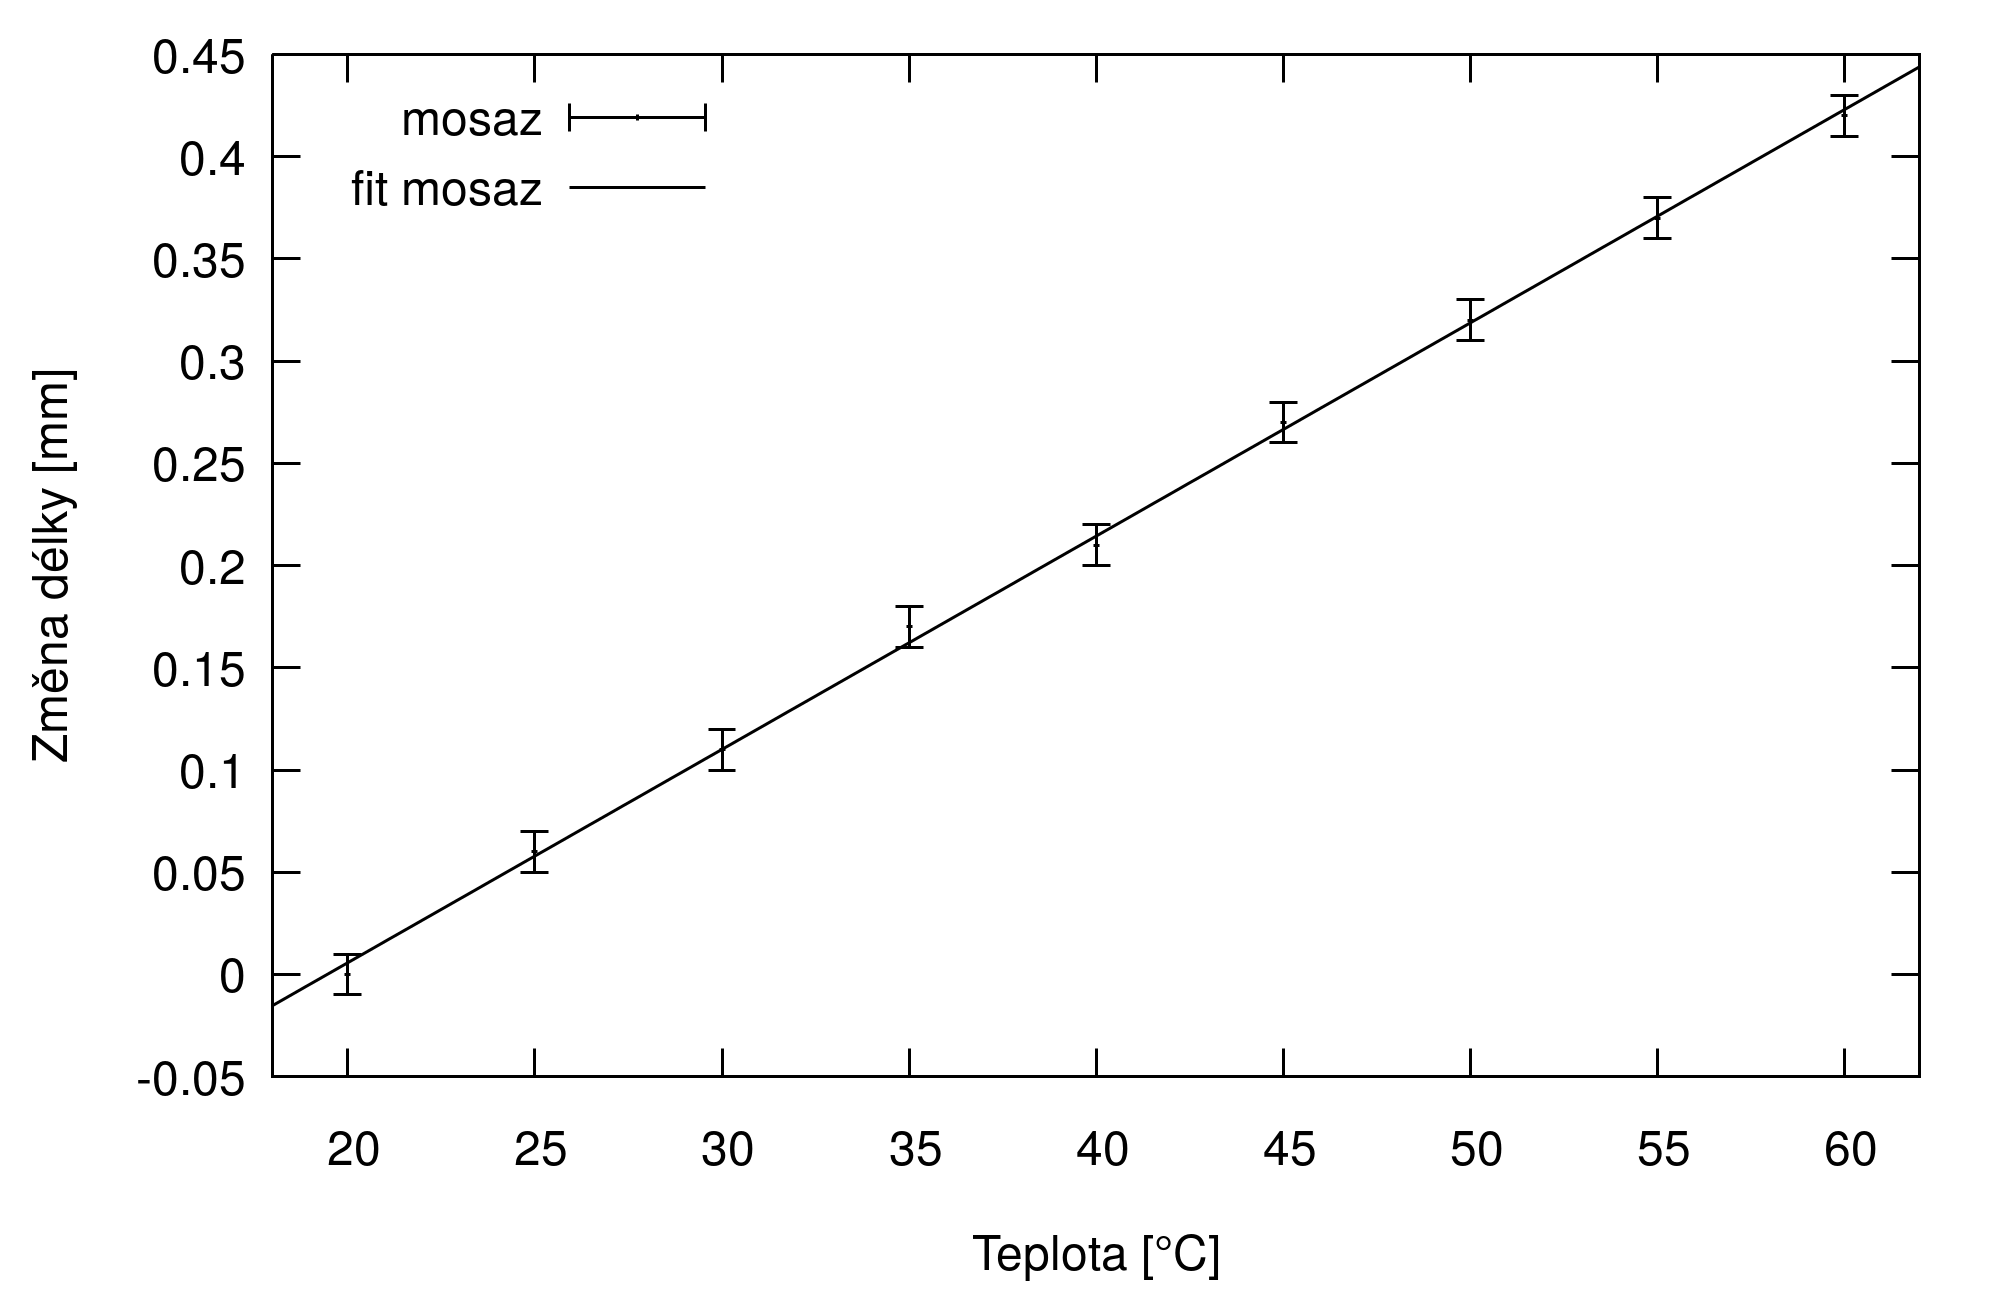
\includegraphics[resolution=350]{roztaznost_mosaz2}
\caption{Graf závislosti délkové roztažnosti mosazi na teplotě}
\end{figure}

\begin{figure}[H]
\centering
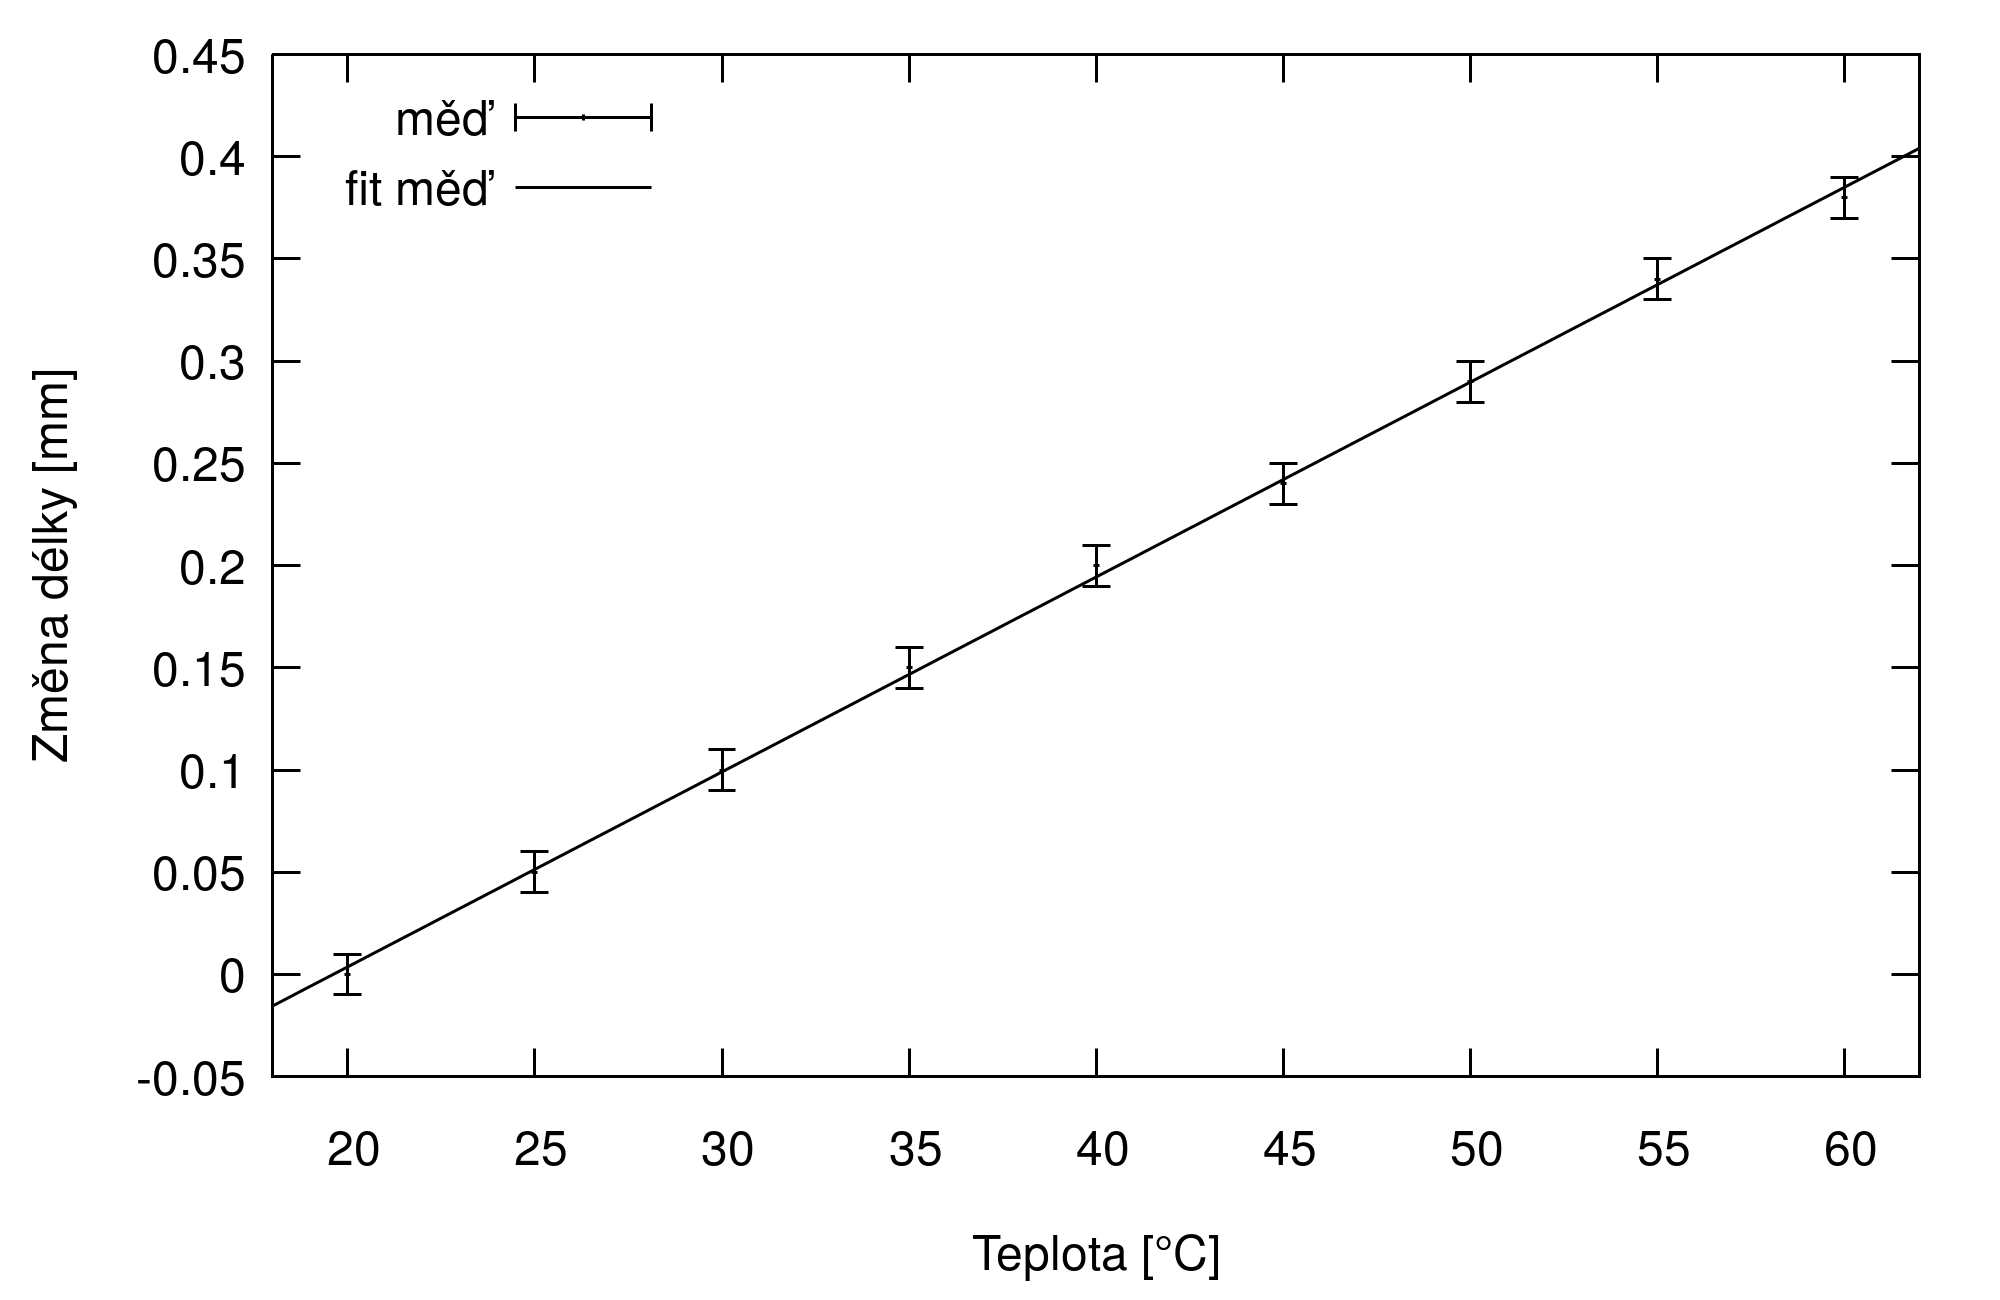
\includegraphics[resolution=350]{roztaznost_med}
\caption{Graf závislosti délkové roztažnosti mědi na teplotě}
\end{figure}

\begin{figure}[H]
\centering
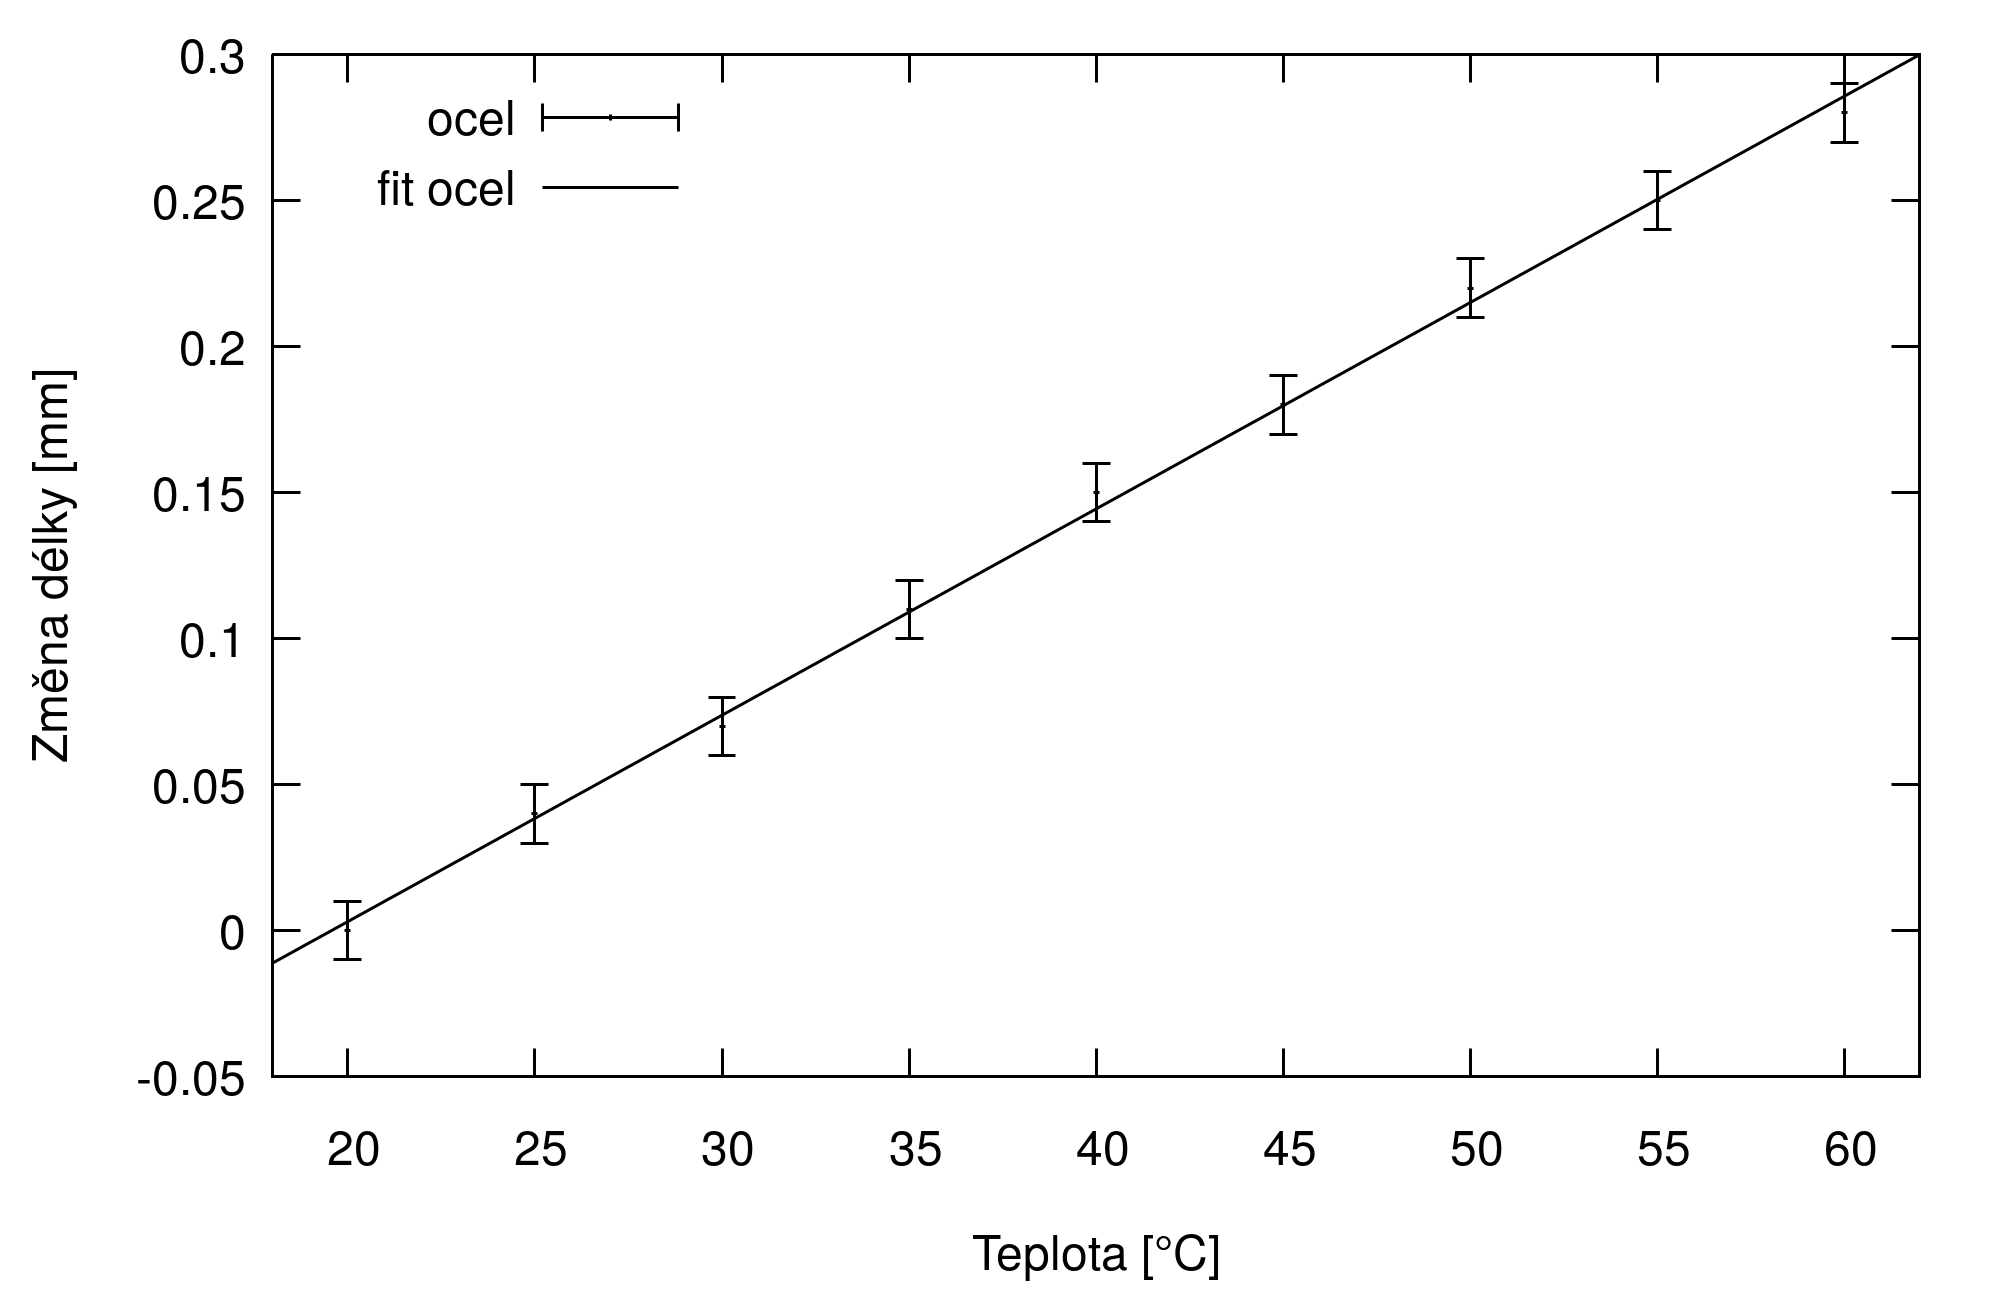
\includegraphics[resolution=350]{roztaznost_ocel}
\caption{Graf závislosti délkové roztažnosti oceli na teplotě}
\end{figure}

\begin{figure}[H]
\centering
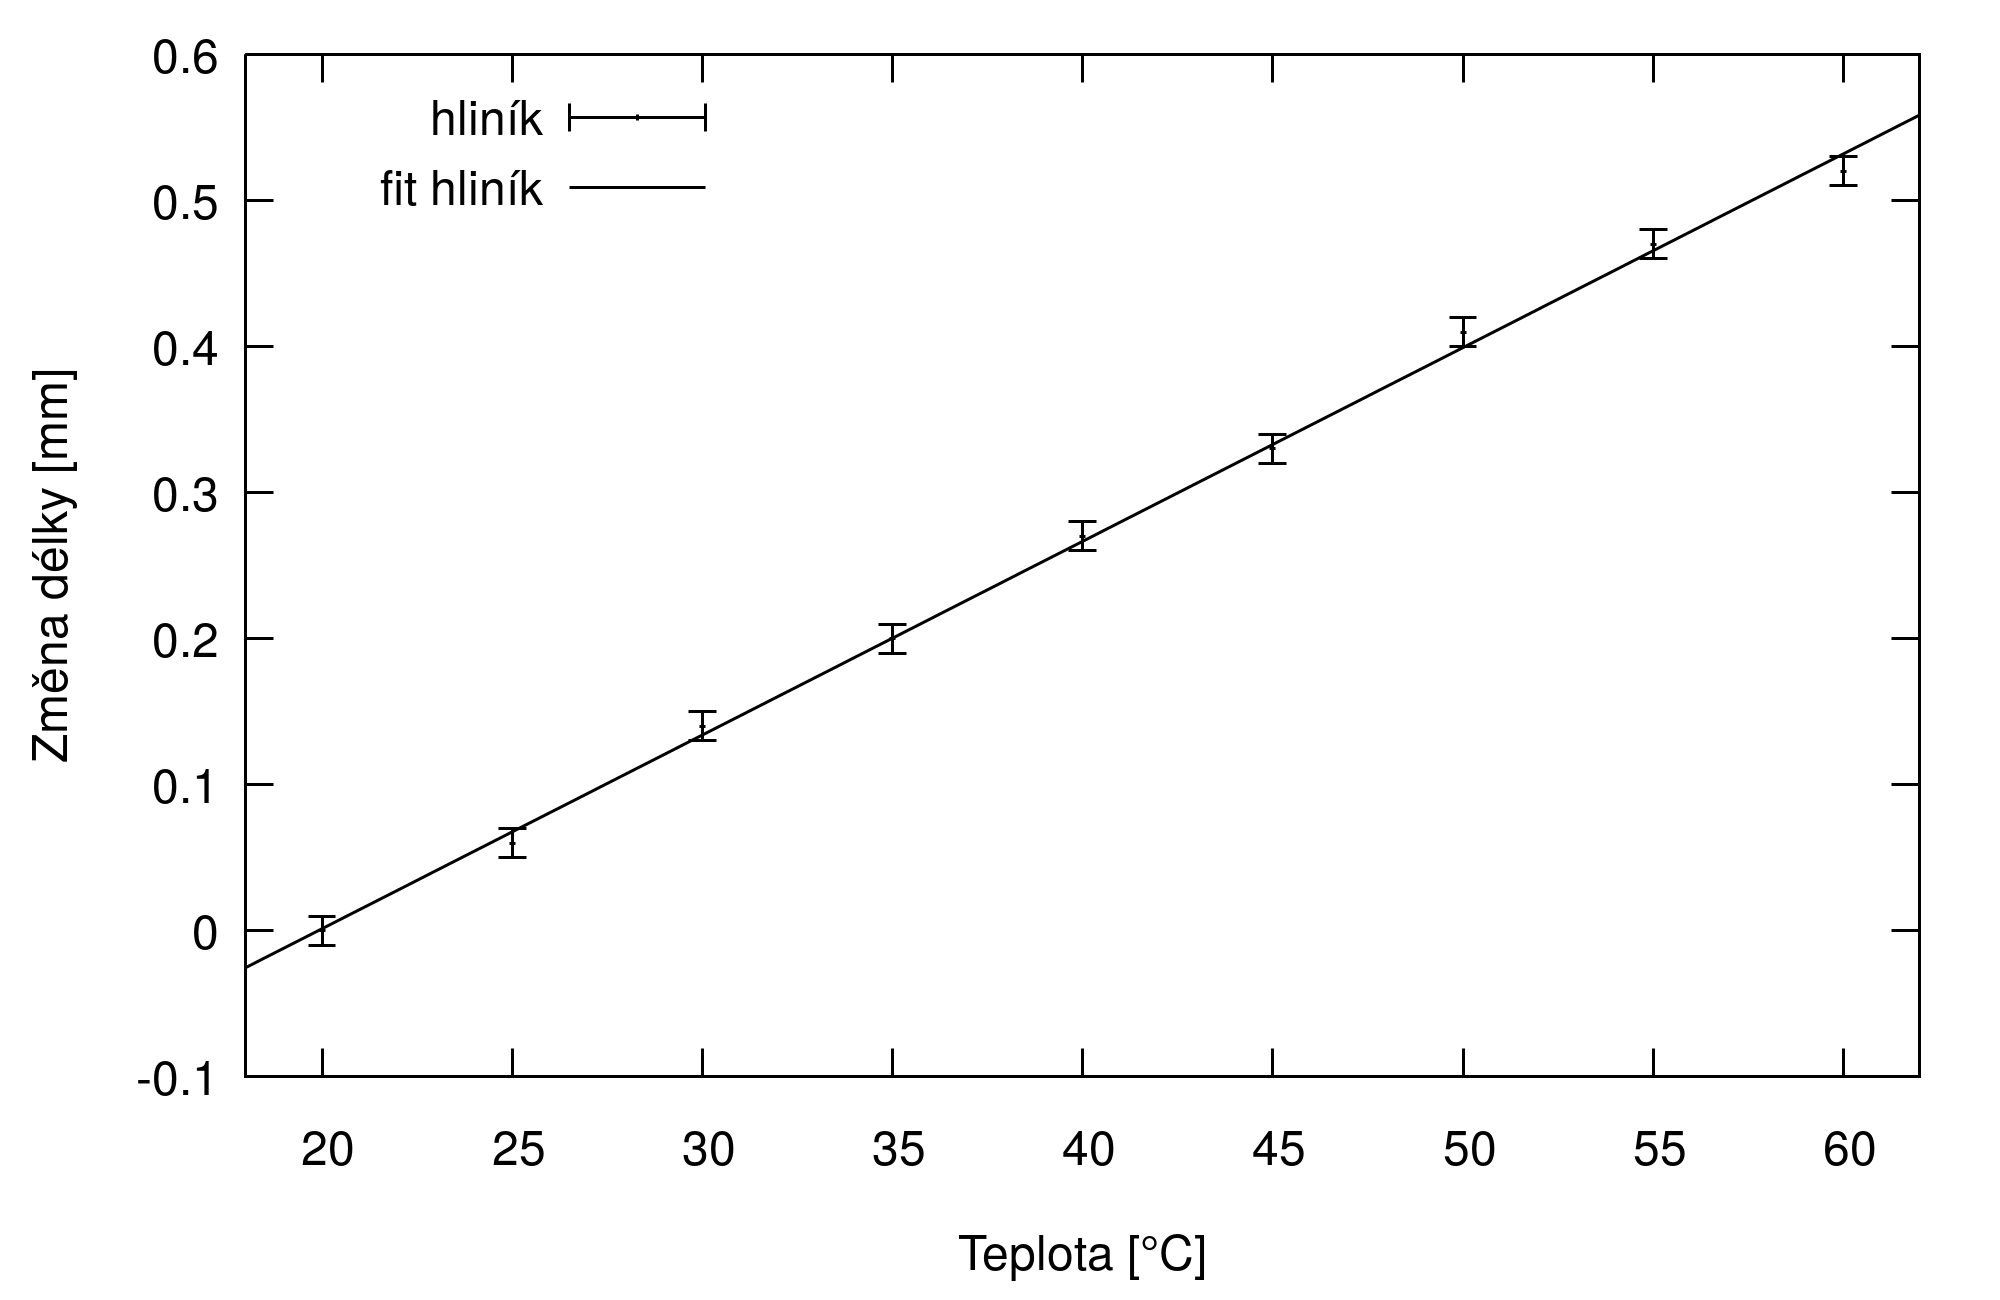
\includegraphics[resolution=350]{roztaznost_hlinik}
\caption{Graf závislosti délkové roztažnosti hliníku na teplotě}
\end{figure}

\begin{table}[H] 
\centering
\setlength{\tabcolsep}{10pt}
\begin{tabular}{cccc}                               \toprule
            &   a       &   b       &   c       \\  \midrule
hodnota     &   0.035   &   -0.034  &   0.007   \\
chyba       &   0.003   &   0.017   &   0.002   \\  \bottomrule
\end{tabular}
\caption{Parametry lineární regrese přímkou $y = kx + q$}
\label{tab:parametry}
\end{table}

\subsection*{Úkol 3}
Dosazením z tabulky \ref{tab:roztaznost} a \ref{tab:parametry} a hodnoty $l$ do \eqref{eq:souc_delka} získáme součinitele délkové roztažnosti
$$ \alpha_{\text{mosaz}}  = (173,3 \pm 1,7) \times \num{e-7} \ \si{\per\kelvin} $$ 	
$$ \alpha_{\text{měď}}    = (158,3 \pm 1,7) \times \num{e-7} \ \si{\per\kelvin} $$
$$ \alpha_{\text{ocel}}   = (118,3 \pm 1,7) \times \num{e-7} \ \si{\per\kelvin} $$
$$ \alpha_{\text{hliník}} = (221,7 \pm 3,3) \times \num{e-7} \ \si{\per\kelvin} $$

Využitím \eqref{eq:vztah_ab} dostaneme součinitele objemové roztažnosti
$$ \beta_{\text{mosaz}}  = (520,0 \pm 5,0)  \times \num{e-7} \ \si{\per\kelvin} $$
$$ \beta_{\text{měď}}    = (475,0 \pm 5,0)  \times \num{e-7} \ \si{\per\kelvin} $$
$$ \beta_{\text{ocel}}   = (355,0 \pm 5,0)  \times \num{e-7} \ \si{\per\kelvin} $$
$$ \beta_{\text{hliník}} = (665,0 \pm 10,0) \times \num{e-7} \ \si{\per\kelvin} $$

\end{document}
